\documentclass{article}
\usepackage[margin=1in]{geometry}
\usepackage{amsmath,amsthm,amssymb}
\usepackage{bbm,enumerate,mathtools}
\usepackage{tikz,pgfplots}
\usepackage{chessboard}
\usepackage[hidelinks]{hyperref}
\usepackage{multicol} % Problem 35

\newenvironment{question}{\begin{trivlist}\item[\textbf{Question.}]}{\end{trivlist}}
\newenvironment{note}{\begin{trivlist}\item[\textbf{Note.}]}{\end{trivlist}}
\newenvironment{references}{\begin{trivlist}\item[\textbf{References.}]}{\end{trivlist}}
\newenvironment{related}{\begin{trivlist}\item[\textbf{Related.}]\end{trivlist}\begin{enumerate}}{\end{enumerate}}


\begin{document}
\rating{3}{1}
Consider figures created out of ``blocks'' starting from some base state and
with the rule that each new block needs to touch as many old blocks as possible.
\begin{figure}[ht!]
  \centering
  \begin{tikzpicture}[
    level distance=2.5cm,
    sibling distance = 3cm,
    level 1/.style={sibling distance=7cm},
    level 2/.style={sibling distance=2.5cm}
  ]
    \node {
      \begin{tikzpicture}[scale=0.6]
        \draw[fill=blue!50, ultra thick] (0,0) rectangle (1,1);
        \draw[fill=blue!50, ultra thick] (1,0) rectangle (2,1);
      \end{tikzpicture}
    }
    child {
      node {
        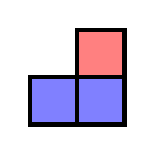
\begin{tikzpicture}[scale=0.6]
          \draw[fill=blue!50, ultra thick] (0,0) rectangle (1,1);
          \draw[fill=blue!50, ultra thick] (1,0) rectangle (2,1);
          \draw[fill=red!50, ultra thick] (1,1) rectangle (2,2);
      \end{tikzpicture}
      }
      child {
        node {
          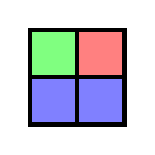
\begin{tikzpicture}[scale=0.6]
            \draw[fill=blue!50, ultra thick] (0,0) rectangle (1,1);
            \draw[fill=blue!50, ultra thick] (1,0) rectangle (2,1);
            \draw[fill=red!50, ultra thick] (1,1) rectangle (2,2);
            \draw[fill=green!50, ultra thick] (0,1) rectangle (1,2);
          \end{tikzpicture}
        }
      }
    }
    child {
      node {
        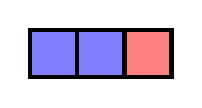
\begin{tikzpicture}[scale=0.6]
          \draw[fill=blue!50, ultra thick] (0,0) rectangle (1,1);
          \draw[fill=blue!50, ultra thick] (1,0) rectangle (2,1);
          \draw[fill=red!50, ultra thick] (2,0) rectangle (3,1);
      \end{tikzpicture}
      }
      child {
        node {
          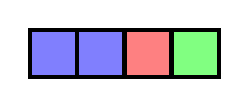
\begin{tikzpicture}[scale=0.6]
            \draw[fill=blue!50, ultra thick] (0,0) rectangle (1,1);
            \draw[fill=blue!50, ultra thick] (1,0) rectangle (2,1);
            \draw[fill=red!50, ultra thick] (2,0) rectangle (3,1);
            \draw[fill=green!50, ultra thick] (3,0) rectangle (4,1);
          \end{tikzpicture}
        }
      }
      child {
        node {
          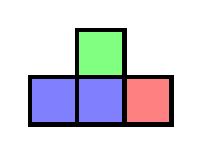
\begin{tikzpicture}[scale=0.6]
            \draw[fill=blue!50, ultra thick] (0,0) rectangle (1,1);
            \draw[fill=blue!50, ultra thick] (1,0) rectangle (2,1);
            \draw[fill=red!50, ultra thick] (2,0) rectangle (3,1);
            \draw[fill=green!50, ultra thick] (1,1) rectangle (2,2);
          \end{tikzpicture}
        }
      }
      child {
        node {
          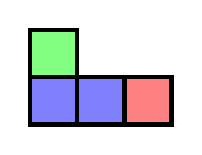
\begin{tikzpicture}[scale=0.6]
            \draw[fill=blue!50, ultra thick] (0,0) rectangle (1,1);
            \draw[fill=blue!50, ultra thick] (1,0) rectangle (2,1);
            \draw[fill=red!50, ultra thick] (2,0) rectangle (3,1);
            \draw[fill=green!50, ultra thick] (0,1) rectangle (1,2);
          \end{tikzpicture}
        }
      }
    };
  \end{tikzpicture}

  \caption{
    On the leftmost path, the final transition is from an ``L'' to a square,
    because the maximum number of faces that can touch is two, so the block must
    be added in the upper left corner.
    Counting the number of vertices gives $a(1) = 1$, $a(2) = 2$, and $a(3) = 4$.
  }
\end{figure}
\begin{question}
  How many distinct figures (up to group action) can be made with $n$ blocks,
  always following a greedy algorithm (with respect to number of faces touching)?
\end{question}

\begin{related}
  \item What if this is done with circles on a hexagonal grid? (Polyiamonds, etc.)
  \item What if this is done in more than $2$ dimensions?
  \item What if the starting shape is different? (e.g. the ``T'' tetromino)
  \item What if the blocks are different? (e.g. dominoes)
  \item What if the constraint is changed? (e.g. each block must touch exactly two sides)
\end{related}

\begin{references}
  \item Problem 75
\end{references}
\end{document}
